\chapter{Training General-Purpose Coding Agents with Constitution Development \textcolor{mediumgreen}{(\textit{proposed})}}
\label{chap:effective-analysis}



\section{Introduction}

In \autoref{chap:hybrid-gym}, we introduce Hybrid-Gym~\cite{hybrid-gym}, which trains a general-purpose coding agent by deriving a set of training task design principles. 
However, \textbf{having proper training tasks is not the only condition for effective coding agent training}.

In addition to training tasks, both Hybrid-Gym and previous work discover other crucial factors of the training outcome.
Most analyses focus on the standard rejection sampling finetuning setting~\cite{rejection-sampling}, where we apply a teacher model to solve a set of problem instances, select successful trajectories by running evaluation, and train the student model on successful trajectories.
In particular, SWE-Gym~\cite{swegym} and SWE-Smith~\cite{swe-smith} find that training instances with a balanced difficulty distribution improve training results.
RepoST~\cite{repost}, SWE-Smith~\cite{swe-smith}, and Hybrid-Gym~\cite{hybrid-gym} demonstrate that it is beneficial to cover diverse repositories in the training data.
Hybrid-Gym~\cite{hybrid-gym} shows that training on trajectories with more steps improves performance.

One of the discoveries from Hybrid-Gym~\cite {hybrid-gym} is that \textbf{even successful trajectories generated from the same set of instances may have substantially different impact in training}.
As shown in \autoref{ablation:self-vs-claude}, we use Claude-Sonnet-3.7 and Qwen2.5Coder-32B to generate successful trajectories on the exact same set of 399 function localization instances and train Qwen2.5Coder-7B on these successful trajectories, separately.
Surprisingly, the model distilled from Claude-3.7 achieves much better performance than the model distilled from Qwen2.5Coder-32B, in terms of the resolved rate, localization rate, and non-empty rate on SWE-Bench-Verified \cite{swebench}.
After manually examining the training trajectories, we observe the following major differences: Claude's trajectories have more reasonable repo-exploration strategies, more thinking, and more solution verification. This indicates that such ``agent behavior patterns'' beyond task success substantially affect training outcome.

Most existing works directly use the latest and most powerful model as the teacher model to construct training data~\cite{swegym,R2EGym,swe-smith,swe-play}, including our Hybrid-Gym work~\cite{hybrid-gym}, which typically cost substantially more than weaker but more cost-efficient models. 
For instance, Claude-Sonnet-3.7 costs \$3.00 per million input tokens, while Qwen2.5Coder-32B only costs \$0.03.
With the ultimate goal of conducting feasible, effective, and generalizable coding agent training, \textbf{we aim to develop a task-agnostic and model-agnostic framework to improve the effectiveness of training trajectories for general coding agent training tasks}. 
By limiting the usage of strong yet expensive models in our pipeline, we reduce the costs of generating training trajectories while maintaining effectiveness.
Furthermore, by revealing the agent behavior patterns in training trajectories that are potentially beneficial or harmful for training outcome, we enable future research to determine the effectiveness of training data before running actual training and evaluation.

In this project, we propose \plusname, a framework that bridges the quality gap between weak and strong teacher models by automatic constitution development.
We first identify beneficial agent behavior patterns (e.g., more systematic repository exploration, solution verification) that are present in strong teacher trajectories but absent in weak teacher trajectories.
Then we derive \emph{constitutions}, a set of concise behavioral guidelines, that can be provided ot the weak teacher model.
The key motivation is that, rather than paying for expensive strong-model inference for every training instance, we can instead identify \emph{what} makes strong trajectories effective and teach the weak model to imitate those behavior patterns, which enables both high-quality and cost-efficient training data generation at scale.


\section{Hypothesis and Preliminary Experiments}
\subsection{Background: Rejection Sampling Finetuning}
\label{plus:sec:preliminary}
Following previous work~\cite{swegym,R2EGym,swe-smith,swe-play,hybrid-gym}, we focus on the rejection sampling finetuning setting~\cite{rejection-sampling}:
To construct the training set, we apply a teacher model to solve a set of problem instances, run evaluation, and collect successful trajectories. 
Then we train a student model on the successful trajectories by supervised finetuning (SFT).
As shown in \autoref{chap:hybrid-gym}, the training tasks do not need to be the same as the downstream tasks in evaluation.

\subsection{Hypothesis}
There could be many differences between strong and weak teacher models' successful trajectories.
Some differences are \emph{task-level patterns} shared across a wide range of examples for the training task---we call these \textbf{problem-solving strategies}.
For example, on the function localization task, a strong model may consistently begin by reading the repository structure before searching for relevant files, while a weak model may directly generate possible file paths without exploring the repository structure.
Other differences are \emph{example-specific}: the exact file paths explored, the precise keywords used in search queries, or the particular lines of code examined. These differences are details that vary with each instance and do not reflect a reusable strategy.
We focus on problem-solving strategy differences because they are shared across many training examples and thus more likely to be transferred to the student model via finetuning.

Our hypothesis is that the strong teacher model employs more robust problem-solving strategies than the weak teacher model, and that these strategies, once embedded in training trajectories, can be learned by the student model through SFT and lead to better distillation performance on downstream tasks.


We show evidence for our hypothesis using two preliminary experiments:

\noindent \textbf{[Preliminary Experiment 1]} We show that on the training dataset, the strong and weak teacher models have different problem-solving strategies. 
On the evaluation dataset, the student agents distilled from the strong and weak teacher models learn similar strategies, which leads to different performances.

\noindent \textbf{[Preliminary Experiment 2]} We show that by adding the corresponding constitutions to the prompt in the training dataset, the weak teacher model produces training trajectories that better follow the desired problem-solving strategies. In addition, training on the new trajectories leads to better distillation performance.

Preliminary experiment 1 shows that problem-solving strategies in the training data can be transferred to student agents and affect the distillation performance.
Preliminary experiment 2 shows that it is possible for the weak teacher model to imitate the strong teacher's problem-solving strategy by developing more effective constitutions.


\subsection{Setup of Preliminary Experiments}
\start{Training and Evaluation Datasets}
In our preliminary experiments, we use the function localization task in the Hybrid-Gym dataset as our training task~\cite{hybrid-gym}, and use the SWE-Bench issue-solving task as the evaluation task~\cite{swebench}.
To save inference cost in evaluation, we sample 50 examples from SWE-Bench Verified that can be resolved by a strong reference model,  Deepseek-v3~\cite{deepseekv3}. We denote this subset as ``SWE-Bench Verified (Easy 50)''. 
As introduced in the Hybrid-Gym paper, models trained on function localization reliably generalize to the issue-solving task, sometimes even outperforming in-domain training.

Following Hybrid-Gym, we report the resolved rates, localized rates, and non-empty rates on SWE-Bench. The localized rate is defined as the percentage of code patches applied to the correct file.

\start{Teacher/Student Models}
We use Qwen2.5Coder-32B~\cite{qwen25coder} as the weak teacher model. We aim to improve the quality of training trajectories it produces.
We use Claude-Sonnet-3.7~\cite{claude37} as the reference strong teacher model. We aim to find the different behavior patterns in the training trajectories generated by the strong and weak teacher models.
We use Qwen2.5Coder-7B~\cite{qwen25coder} as the student model.





\subsection{Preliminary Experiment 1: Problem-Solving Strategies Affect Distillation Performance}
\start{Experimental Method}
We apply Claude-Sonnet-3.7 and Qwen2.5Coder-32B to the same set of function localization instances and collect their successful trajectories on 399 overlapping instances.

As shown in the upper left part of \autoref{fig:plus:framework}, to find the differences between the strong and weak teacher models' problem-solving strategies, we first apply an LLM (o3-mini~\cite{o3_mini}) to identify a list of potential differences between each pair of trajectories generated by the strong and weak teacher models. Then we call o3-mini again to summarize the pattern of different agent behavior patterns.
We manually identify the differences in problem-solving strategies (e.g., the strong model tends to locate functions by keywords while the weak model tends to locate functions by reading the whole file) and design quantitative features for each difference (e.g., we measure the frequency of the ``keyword searching inside files'' actions by matching regular expression patterns).

Finally, we train two Qwen2.5Coder-7B student models, one on each teacher's trajectory set, using the same SFT procedure. We evaluate the models on SWE-Bench Verified (Easy 50) and compare the features of the two student models' evaluation trajectories. We focus on the evaluation examples where the student agent trained on the strong teacher model's trajectories solves the task but the weak student agent does not.


\begin{table}[t]
  \centering
  \small
  \begin{tabular}{l cc}
  \toprule
  \bf Features & \bf Qwen-32B & \bf Claude-3.7 \\
  \midrule
  In-file keyword searching actions (\%) & \bad 6.7  & \good 20.2 \\
  Think actions (\%)                     & \bad 0.0  & \good 6.9  \\
  Read file before editing (\%)          & \bad 83.1 & \good 99.7  \\
  \bottomrule
  \end{tabular}
  \caption{Frequency of agent behavior features in the teacher models' successful trajectories on the function localization training task. Claude-3.7 uses in-file keyword search more, thinks more, and almost never edits a file without reading it first.}
  \label{tab:plus:prelim1-train}
  \end{table}
  
  \begin{table}[t]
  \centering
  \small
  \resizebox{\columnwidth}{!}{%
  \begin{tabular}{l cc cc}
  \toprule
  \multirow{2}{*}{\bf Features} &
  \multicolumn{2}{c}{\bf Divergent Subset} &
  \multicolumn{2}{c}{\bf SWE-Bench Verified (Easy 50)} \\
  \cmidrule(lr){2-3} \cmidrule(lr){4-5}
  & Student of Qwen-32B & Student of Claude-3.7 & Student of Qwen-32B & Student of Claude-3.7 \\
  \midrule
  In-file keyword searching actions (\%) & \bad 5.3  & \good 17.9 & \bad 11.8 & \good 27.0 \\
  Think actions (\%)                     & \bad 0.0  & \good 6.3  & \bad 0.0  & \good 3.6  \\
  Read file before editing (\%)            & \good 99.0  & \good 99.3  & \good 95.9  & \good 96.9  \\
  \bottomrule
  \end{tabular}%
  }
  \caption{Frequency of agent behavior features in the student models' evaluation trajectories on SWE-Bench Verified (Easy 50). ``Diff-subset'' refers to the examples where the Student of Claude-3.7 succeeds but the Student of Qwen-32B fails. The student models inherit the teacher's strategies in training trajectories.}
  \label{tab:plus:prelim1-eval}
  \end{table}



\start{Experimental Results}
As shown in \autoref{tab:plus:prelim1-train} and \autoref{tab:plus:prelim1-eval}, we observe the following results:

\noindent(1) The strong and weak teacher models have different problem-solving strategies in the training data.
Particularly, Claude-3.7 performs in-file keyword searching 3$\times$ more frequently than Qwen-32B (20.2\% vs.\ 6.7\%), includes explicit thinking actions in 6.9\% of steps while Qwen-32B never does, and almost always reads a file before editing it (99.7\% vs.\ 83.1\%).

\noindent(2) The student models learn the problem-solving strategies from their respective teacher models.
Particularly, the Student of Claude-3.7 uses in-file keyword searching more than twice as often as the Student of Qwen-32B (27.0\% vs.\ 11.8\% on the full evaluation set), and retains the thinking behavior (3.6\% vs.\ 0.0\%), closely mirroring the gap observed in the teacher trajectories.

\noindent(3) On the divergent subset where the strong student resolves the task but the weak student does not, the strategy gap between the two students is even more pronounced.
The Student of Claude-3.7 uses keyword searching in 17.9\% of steps vs.\ 5.3\% for the Student of Qwen-32B, and thinks in 6.3\% of steps vs.\ 0.0\%.
This indicates that the strategy differences inherited from the teacher are a key driver of the performance gap: when the strong student succeeds and the weak student fails, the strong student is more likely to be actively employing the superior problem-solving strategies learned from Claude-3.7's trajectories.



\begin{figure}[t]
  \centering
  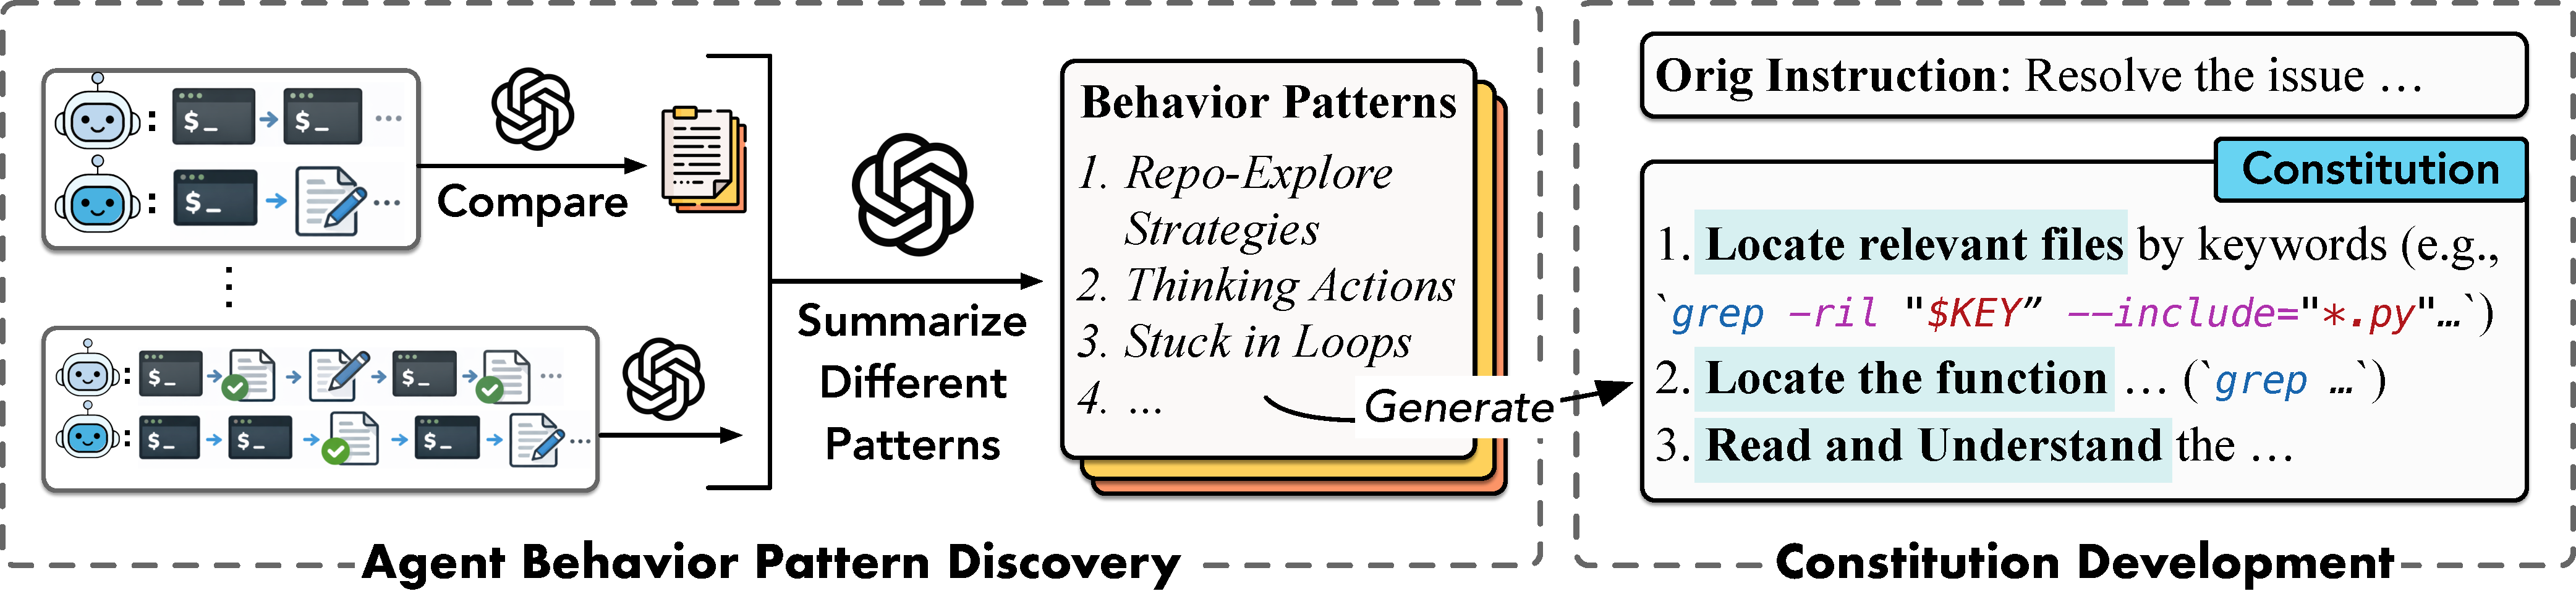
\includegraphics[width=\textwidth]{plus_figs/prelim_method.pdf}
  \caption{The preliminary version of our framework, as used in \textbf{Preliminary Experiment 2}. We denote it as \plusname-v0.  
  We first discover the different behavior patterns in the strong and weak teacher models' successful trajectories. Then we manually write a detailed constitution based on the differences. Finally, we train a student model on the new training trajectories.
  }
  \label{fig:plus:prelim-method}
  \end{figure}


\begin{figure}[t]
  \centering
  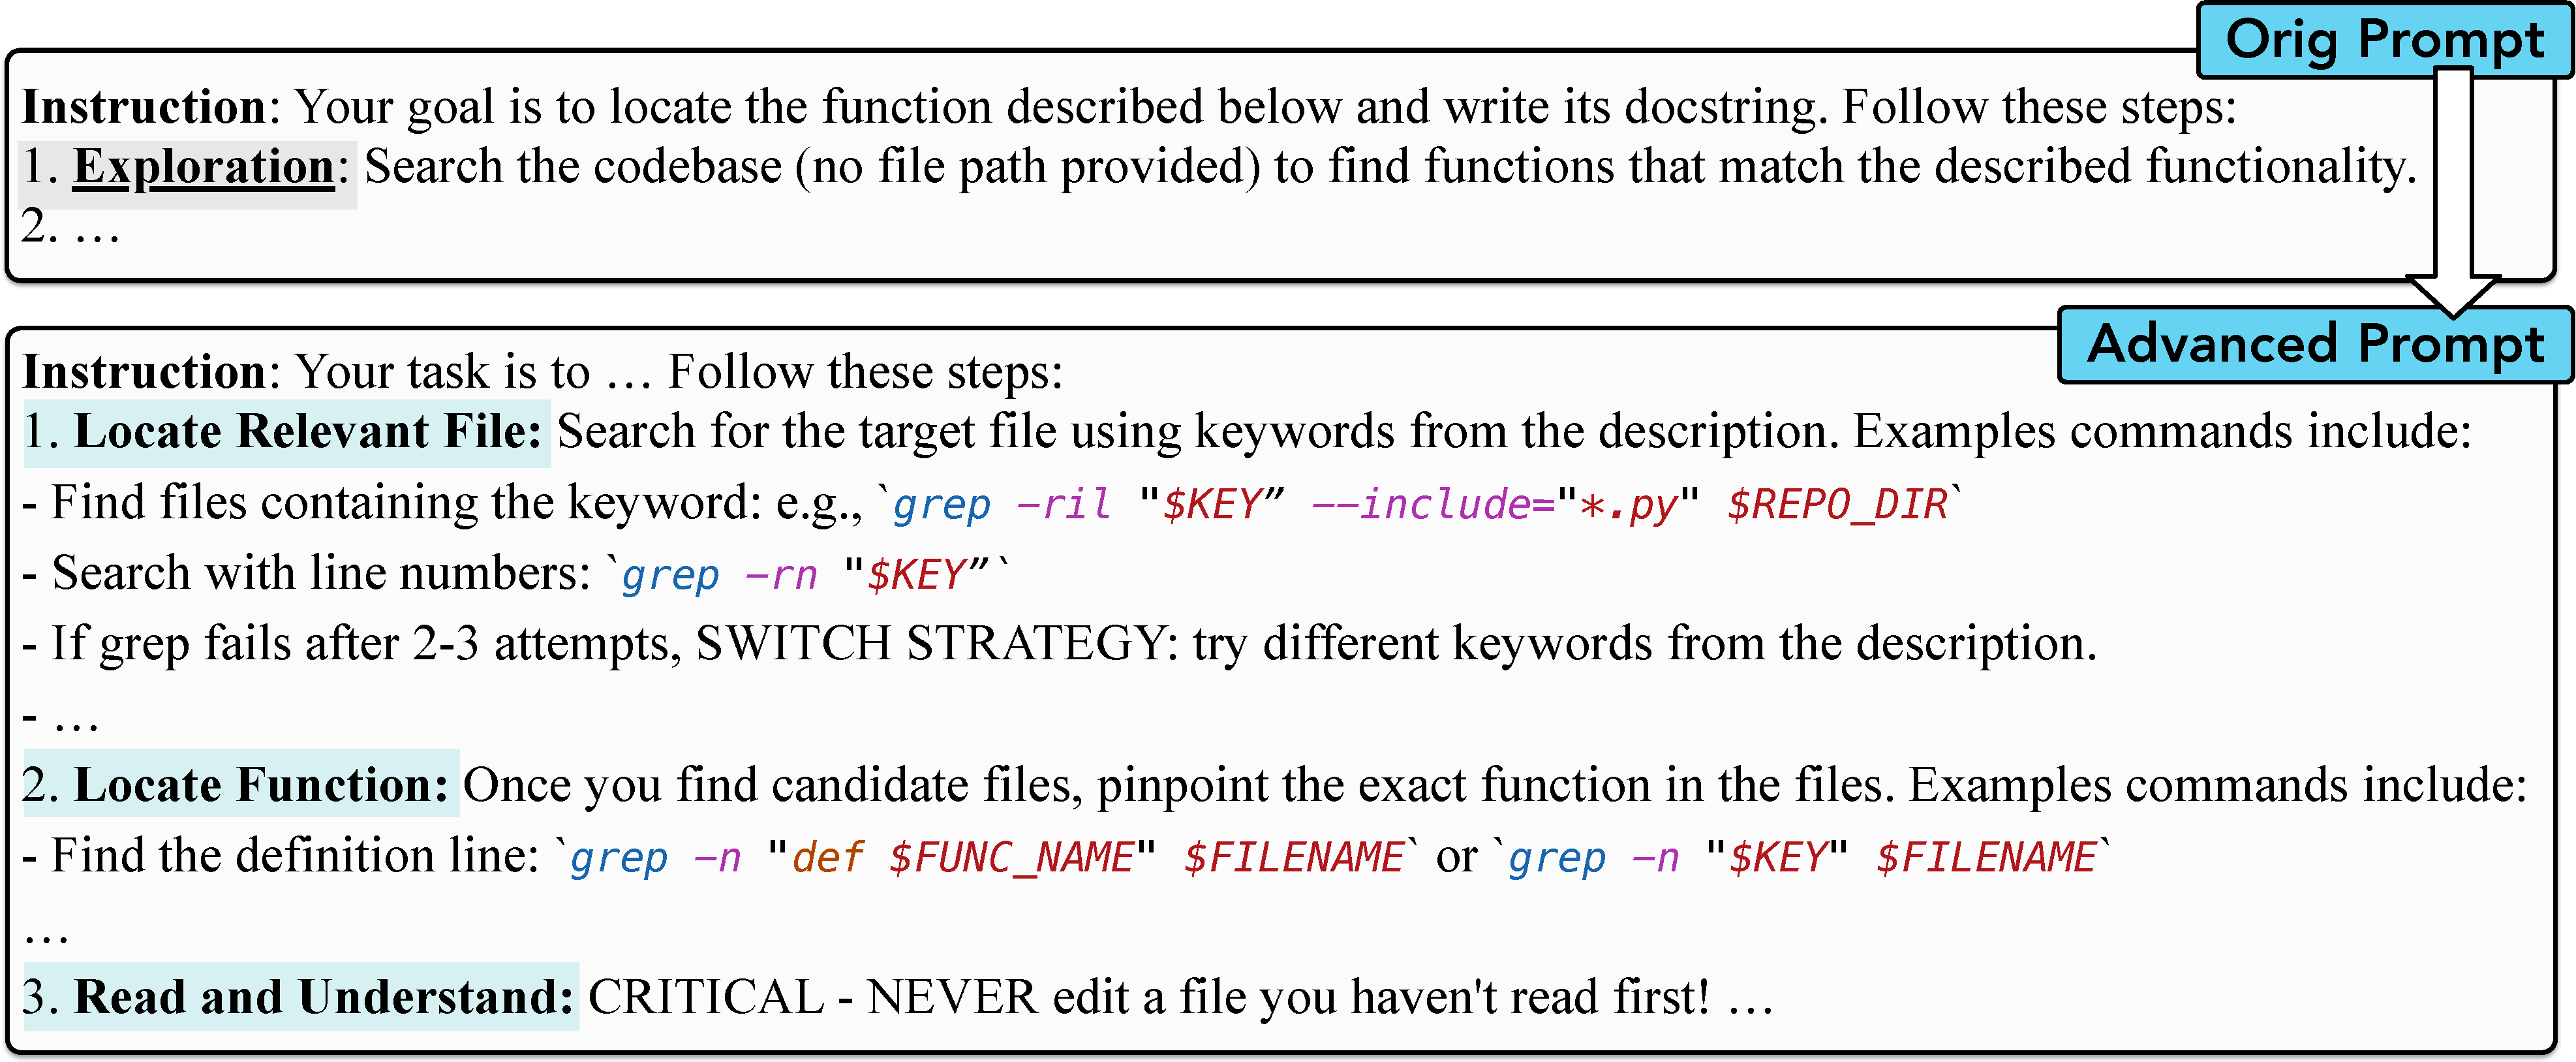
\includegraphics[width=\textwidth]{plus_figs/preliminary.pdf}
  \caption{The constitution we use for the preliminary experiments, which encodes the agent behavior patterns that are present in the strong teacher trajectories but absent in the weak teacher trajectories.}
  \label{fig:plus:preliminary}
\end{figure}


\begin{table}[t]
\centering
\small
\resizebox{0.9\columnwidth}{!}{%
\begin{tabular}{l ccc}
\toprule
\multirow{2}{*}{\bf Teacher Model (|Train Size|)} &
\multicolumn{3}{c}{\bf SWE-Bench Verified (Easy 50)} \\
\cmidrule(lr){2-4}
& Resolved \% & Localized \% & Non-Empty \% \\
\midrule
\sdlrow & \multicolumn{3}{c}{\textit{Base Model: Qwen2.5Coder-7B}} \\
\midrule
\textemdash & \worse 2.0 & 4.0 & 8.0 \\
\midrule
Qwen2.5Coder-32B (399) & \bad 4.0 & 20.0 & 48.0 \\
Qwen2.5Coder-32B + \plusname-v0 (399) & \good 8.0 & 46.0 & 68.0 \\
Claude-Sonnet-3.7 (399)   & \better \bf 26.0 & 68.0 & 86.0 \\
\bottomrule
\end{tabular}%
}
\caption{Results on training Qwen2.5Coder-7B on successful trajectories of the exact same 399 function localization instances generated by Claude-3.7, Qwen2.5Coder-32B, and Qwen2.5Coder-32B with the constitutions we develop in the preliminary experiments (denoted as + \plusname-v0). 
We evaluate the student models on a subset of the SWE-bench Verified issue-solving dataset after training. 
}
\label{ablation:self-vs-claude}
\end{table}


\subsection{Preliminary Experiment 2: Problem-Solving Strategies can be Guided by Constitutions}
\start{Experimental Method}
After observing that the strong and weak teacher models have different problem-solving strategies, which lead to different distillation performances, we conduct [Preliminary Experiment 2] to investigate whether it is possible for the weak teacher model to imitate the strong teacher's problem-solving strategy by developing more effective constitutions.

As shown in \autoref{fig:plus:preliminary}, we manually write a detailed constitution that encodes the problem-solving strategies that are present in the strong teacher trajectories but absent in the weak teacher trajectories.
We then add the constitution to the prompt of the weak teacher model when generating training trajectories.
Similarly, we train a Qwen2.5Coder-7B student model on the new training trajectories and evaluate the model on SWE-Bench Verified (Easy 50).

\start{Experimental Results}
As shown in \autoref{ablation:self-vs-claude}, we observe the following results:

\noindent(1) The student model trained on the new training trajectories (denoted as + \plusname-v0) performs better than the student model trained on the original training trajectories (denoted as Qwen2.5Coder-32B).
Particularly, the student of Qwen-32B + \plusname-v0 achieves 8.0\% resolved rate, 46.0\% localized rate, and 68.0\% non-empty rate, while the student model trained on the original training trajectories achieves 4.0\% resolved rate, 20.0\% localized rate, and 48.0\% non-empty rate.
This indicates that the constitution is effective in guiding the weak teacher model to produce training trajectories that better follow the strong teacher's problem-solving strategy.

\noindent(2) However, even with the new constitution, there is still a gap between the weak and strong teacher's distillation performances.
The student of the strong teacher model (Claude-3.7) achieves 26.0\% resolved rate, 68.0\% localized rate, and 86.0\% non-empty rate, which is still substantially higher than the student of Qwen-32B + \plusname-v0.
We will discuss the limitations of the preliminary experiments in \S\ref{plus:sec:limpreliminary}.




\subsection{Limitations of Preliminary Experiments}
\label{plus:sec:limpreliminary}
While the preliminary experiments demonstrate the promise of constitution-guided training trajectory generation, they also reveal three limitations that motivate our proposed framework.

\start{Limitation 1: Incomplete coverage of agent behavior patterns.}
The constitutions in our preliminary experiments may not cover all salient behavior patterns that differ between the strong and weak teacher models.
To discover more salient behavior patterns, we propose to (1) iteratively run the framework of behavior pattern discovery, constitution development, and verification, and (2) improve the behavior pattern discovery step with non-LLM methods. Specifically, we plan to first convert the trajectories into more abstract sequences (e.g., by summarizing the purposes of each action, or by extracting the action type of each action). Then we apply clustering algorithms to discover different patterns in the strong and weak teacher models' sequences.


\start{Limitation 2: Poor instruction following.}
Even if the constitutions are perfect, it is still possible that the weak teacher agent does not fully follow the constitutions. 
To address this limitation, we propose to iteratively refine the constitutions and check whether the new training trajectories follow the desired behavior patterns.
Specifically, we create a ``gradebook'' to measure each behavior pattern using an automatic metric (e.g., the frequency actions that search for keywords inside files). A metric is effective if it can distinguish the strong and weak teacher models' trajectories.
Then we iteratively refine constitutions, generate new training trajectories, and use the gradebook to check whether the new training trajectories follow the desired behavior patterns.


\start{Limitation 3: Imperfect desired behavior pattern distillation.}
Finally, even when the desired behavior patterns are present in the training trajectories, it is still possible that the student model fails to fully learn them through SFT alone.
Addressing this limitation (e.g., by using stronger student models or more advanced training methods) is out of the scope of this project, and we leave it to future work.



\section{Proposed Methodology: the \plusname Framework}
As shown in \autoref{fig:plus:framework}, with a strong teacher model as reference, we propose an \textbf{automatic} framework to iteratively discover the beneficial and harmful agent behavior patterns and develop constitutions to guide the weak teacher model to produce more effective training trajectories.
In particular, we first identify the differences between their behaviors in successful trajectories (\S\ref{plus:sec:discovery}).
Then we develop constitutions to reflect the desired behavior patterns. We iteratively refine the constitutions until it reflects the desired behavior patterns in the training trajectories (\S\ref{plus:sec:augmentation}).
Finally, we determine whether our constitutions are effective by training a student model on the updated trajectories (\S\ref{plus:sec:verification}).
The above steps can be iteratively adopted.





\subsection{Agent Behavior Discovery}
Our analysis in \autoref{ablation:self-vs-claude} shows that agent behavior patterns beyond task success substantially affect training performance. 
The first question to ask is: \textbf{what are the different behavior patterns in strong and weak teacher models' trajectories?}
To answer this question, we first adopt an LLM (e.g., o3-mini~\cite{o3_mini}) to identify a list of potential differences between the trajectories generated by the strong teacher model and the weak teacher model.
Then we manually design statistical analyses to verify that these differences exist.

\label{plus:sec:discovery}
\start{Agent Behavior Pattern Discovery}
As shown in \autoref{fig:plus:framework}, we start by applying the strong and weak teacher models on the same set of training instances and collect the instances where both of them generate a successful trajectory.
To compare their behavior patterns when resolving the same task, we apply an LLM to conduct pairwise comparisons and identify the differences in each pair of trajectories, in terms of both the high-level problem-solving strategy and the concrete actions.
Finally, after gathering the differences on a small set of trajectory pairs (we use 30 pairs in our experiments), we apply an LLM again to summarize the pattern of different agent behaviors.

An example of differences in concrete actions is that Claude-3.7 calls the ``think'' action significantly more often than Qwen2.5Coder-32B.
As for high-level strategies, we observe that Claude-3.7~\cite{claude37} adopts different repo-exploration strategies from Qwen2.5Coder-32B~\cite{qwen25coder}. 
Claude-3.7 typically follows the steps of locating relevant Python files by several keywords, locating the concrete functions or classes inside those files by another round of keyword searching, understanding the functionality and usage of the located functions, and finally searching for potential test files.
In comparison, after searching for relevant files with keywords, Qwen2.5Coder-32B~\cite{qwen25coder} directly reads the whole file to locate relevant functions. It never tries to understand the functionality and usage of the functions and never searches for test files.

\start{Gradebook Generation}
After identifying salient trajectory behavior patterns, we develop a ``gradebook'' that quantifies each behavior pattern using an automatic metric.

We provide an example in \autoref{fig:plus:framework}, where we break down repo-exploration strategies into quantitative terms.
For instance, we check whether the agent locates functions by keyword searching by matching the following Regular Expressions (RE) patterns: \textit{grep -n ``def \$FUNC'' \$FILE}, \textit{grep -n ``class \$CLASS'' \$FILE}, and \textit{grep -n ``\$KEYWORD'' \$FILE}.


\begin{figure}[t]
\centering
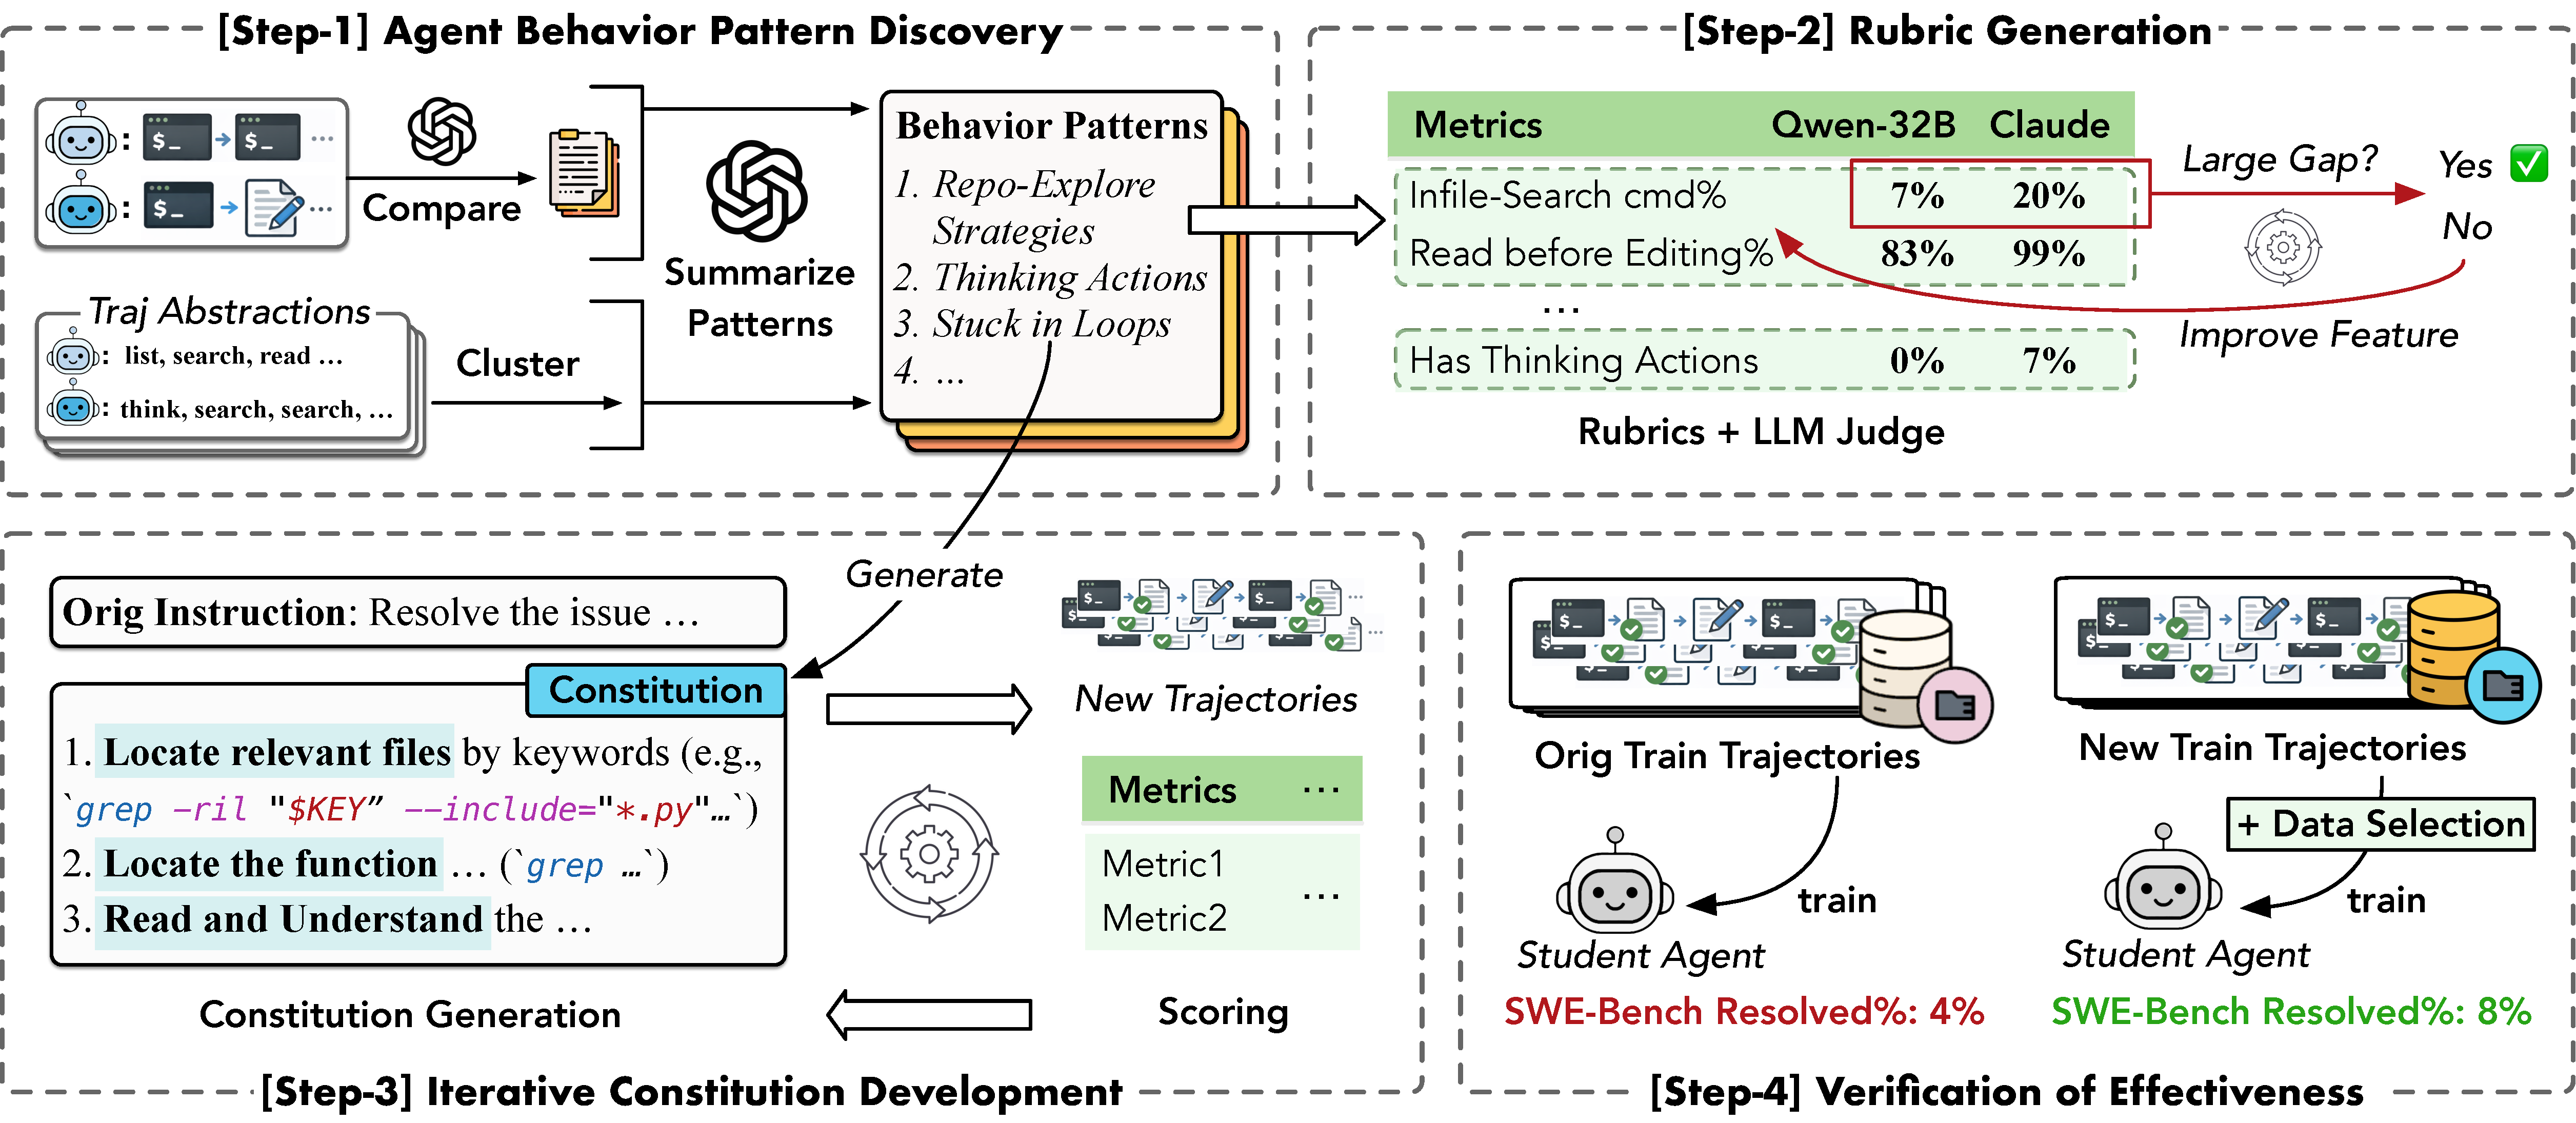
\includegraphics[width=\textwidth]{plus_figs/hybridplus.pdf}
\caption{The \plusname framework. Compared to the preliminary version (\autoref{fig:plus:prelim-method}), we:
(1) improve behavior pattern discovery by abstracting the trajectories and clustering them into different patterns.
(2) iteratively refine the constitutions by generating new training trajectories and checking with a ``gradebook'', which contains a set of quantifiable metrics to measure each behavior pattern.
(3) iteratively run step 1 to 4 to discover more salient behavior patterns.
}
\label{fig:plus:framework}
\end{figure}




\subsection{Constitution Development}
\label{plus:sec:augmentation}

In \S\ref{plus:sec:discovery}, we find a list of different behavior patterns in the strong and weak teacher models' trajectories.
Here we \textbf{develop constitutions to imitate the strong model's behavior patterns in the weak model's trajectories}.

\start{Constitution Generation}
The most straightforward method is to improve the task prompt in training by adding a list of rules, which are called ``constitutions'' in previous research~\cite{constitutional-ai}.
Here we adopt Constitutional AI's method~\cite{constitutional-ai} that writes the constitution, generates a few examples, uses an LLM to judge whether the constitutions are well satisfied, and refines the prompts, if needed.

\autoref{fig:plus:framework} shows an example of the constitutions we develop. 
The original rollout prompt is concise about repo-exploration: ``explore the codebase to find functions that match the described functionality''. 
After observing that Claude-3.7 has additional function searching, function understanding, and test function searching steps compared to Qwen2.5Coder-32B, we expand the original instruction with a list of specific steps: locate relevant files by keywords, locate functions by keywords, read the functions, etc.. We also equip each step with several patterns of concrete actions that the agent can follow (e.g., searching for keywords using the ``\textit{grep}'' command).


\start{Iterative Constitution Refinement}
A single round of constitution writing may not be sufficient to fully reflect the desired behavior patterns in the training trajectories.
We therefore adopt an iterative refinement procedure: after generating a new set of training trajectories with the current constitutions, we run the gradebook from \S\ref{plus:sec:discovery} to measure how well the desired behavior patterns are reflected.
If the target behavior patterns are not yet sufficiently present---or if new behavioral gaps surface---we revise the constitutions accordingly and repeat the rollout.
This loop continues until the gradebook scores of the augmented weak teacher trajectories are close to those of the strong teacher, or until no further improvement is observed.



\subsection{Verification of Effectiveness}
\label{plus:sec:verification}
In \S\ref{plus:sec:discovery} and \S\ref{plus:sec:augmentation}, we discover the different behavior patterns in the strong and weak teacher models' trajectories and use three approaches to imitate the strong model's behavior patterns in the weak model's training trajectories.
To examine the effectiveness of our approaches, we first verify that the desired behavior patterns are indeed present in the augmented trajectories by running the statistical analyses introduced in \S\ref{plus:sec:discovery}.
After that, we train a student model on the original and augmented trajectories, separately, and observe the differences in the training performances.

If training on augmented trajectories yields better performance, we record the corresponding agent behaviors and approaches.
\textbf{The outcome of the \plusname framework will include: (1) a list of beneficial or harmful agent behavior patterns in training trajectories, and (2) a list of approaches to add or remove them from a weak teacher model's trajectories.}

Finally, we go back to the first step: agent behavior pattern discovery (\S\ref{plus:sec:discovery}) and iteratively run the framework to find the remaining agent behavior patterns that are salient to training outcome.






\section{Proposed Experiments}
To showcase that our work provides a better understanding of coding agent training, we aim to show that training with the trajectories generated by \plusname has better distillation performance than training with the original trajectories and with lower cost than training on the strong model's trajectories.


\yiqing{New proposed experiments}

We want to study the following research questions:

(1) Can we discover the behavior patterns in training trajectories that affect training effectiveness? (already partially reached by the preliminary experiment)

(2) Can we improve trajectory effectiveness by constitution development (already partially reached by the preliminary experiment)

(3) Are the constitutions model-agnostic and task-agnostic? (open research question)



\subsection{Proposed Experimental Setup}
\start{Training Datasets and Teacher/Student Models}
To show that our method is task-agnostic, we apply the \plusname framework on five training tasks: the SWE-Gym issue-solving task~\cite{swegym} and the four tasks in the Hybrid-Gym dataset: function localization, issue localization, dependency search, and function generation~\cite{hybrid-gym}.

To show that our method is model-agnostic, we experiment on two weak teacher models: Qwen2.5Coder-32B~\cite{qwen25coder} and GLM-4.7-Flash~\cite{GLM-4.7}. We only experiment with one strong teacher model: Claude-3.7~\cite{claude37} to save the cost.

Following Hybrid-Gym~\cite{hybrid-gym}, we conduct experiments with two student models: Qwen2.5Coder-7B and Qwen2.5Coder-32B.

\start{Evaluation Datasets and Metrics}
With the goal of training general-purpose coding agents, we follow Hybrid-Gym~\cite{hybrid-gym} and conduct multi-task evaluation on the SWE-Bench issue-solving benchmark~\cite{swebench}, the SWT-Bench test generation benchmark~\cite{swt-bench}, and the Commit-0 library generation benchmark~\cite{commit0}.

We report the resolved rates on the three datasets and additionally report the localized rate on SWE-Bench: the percentage of code patches applied to the correct file, and the non-loop rate: the percentage of trajectories without any ``loops'', which is defined as repeating the same action three times consecutively~\cite{swegym}.

To evaluate the cost-efficiency of our method, we further record the cost we spend on generating training trajectories for each method.


\subsection{Proposed Experiments and Expected Results}
For each training dataset, we will compare the performances of the three sets of training sets: (1) trajectories generated by the strong teacher model, 
(2) trajectories generated by the weak teacher model, and 
(3) the weak teacher model's trajectories generated from the constitutions we obtain using the \plusname framework.

Then we train the student model on these three training sets, separately. We expect to see that: training with weak teacher model's trajectories based on \plusname constitutions 
(1) has better performance than training with the original trajectories and 
(2) has lower cost than training on the strong model's trajectories.


\section{Proposed Future Work}
In addition to this proposed project, our discovery about the significance of agent behavior patterns beyond task success also has important implications for future research.

One direction is to develop more advanced training methods so that the problem-solving strategies can be better distilled into the student agent.
For instance, in training, we can assign higher weights to the actions that reflect the strategies we need the student agent to learn.
Furthermore, in this work, we only experiment with the supervised finetuning setting. Future work may also develop their training methods based on other training paradigms, such as reinforcement learning.

Another direction is to design evaluation metrics beyond correctness, which are not captured by most current benchmarks. 
In our preliminary experiments, we find that even without a systematic exploration of the repository, a model could still resolve an issue by accidentally opening the correct file through a random guess. 
To have a more comprehensive evaluation of model capability, future work may design evaluation aspects and metrics that distinguish such ``success by random guess'' behaviors from real success.